\documentclass[a4paper,12pt]{article}
\usepackage[italian]{babel}
\usepackage[utf8]{inputenc}
\usepackage{graphicx}
\usepackage{listings}
\usepackage{color}
\usepackage[usenames,dvipsnames,svgnames,table]{xcolor}

\title{Guide to Raven Code}
\author{Marco Baruzzo, elbaru90@gmail.com}

\begin{document}
	\maketitle

	\titlepage

	\tableofcontents
	\newpage

	\section{Installation}
		Raven Code prerequisites:
		\begin{itemize}
			\item ROOT 6.10
			\item Python 2.7 (only for GUI)
			\item Kivy 1.9.6 (only for GUI)
		\end{itemize}
		Raven Code doesn't need a particular installation, if in the PC are installed all the prerequisites it will work.

	\section{Use}
		\subsection{Checking the mappings}
			The first things to do is check or modify the PAD and APV mapping in the specific file (respectively \textit{apv\_mapping\_hybrid} and \textit{detector\_mapping\_hybrid}).\\ 
			In the file, firstly, we find the dimensions of the APV surface in terms of PAD with row per columns logic (for example 16 PAD x 8 PAD, 16 row and 8 columns), after there is the PAD order, from top to bottom and from left to right.\\
			\begin{minipage}[c]{0.49\textwidth}
				For example this:\\
				\centering
				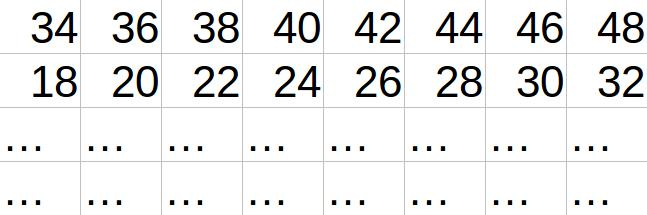
\includegraphics[scale=0.3]{mapping.png}
			\end{minipage}
			\begin{minipage}[c]{0.49\textwidth}
				\centering
				became:\\
				34\\
				36\\
				38\\
				40\\
				42\\
				44\\
				46\\
				48\\
				18\\
				20\\
				22\\
				24\\
				26\\
				28\\
				30\\
				32\\
				...\\
			\end{minipage}
			The Detector mapping works in the same way, in particular with PADs became APVs and AVP became Detector.
		\subsection{Use with Graphical Interface} 
			Raven Code can be opened with a double click on the \textit{Raven\_Code.sh} file or from terminal, it will open the GUI and a terminal window.
			The GUI is divided in 4 sections and following the interface from top to bottom a complete analysis can be done.
			To start the analysis it's enough to complete all fields and press the gray buttons from top to bottom.
			When the work in a section is complete the red line will change color to green.
			You can also follow the program output in the terminal window.
			Some fields will auto-complete but, if you want, you can change the values.\\
			TIPS:
			\begin{itemize}
			 	\item The fast way to use it is opening the folder that contains the raw file and copy the file in the fillable field;
			 	\item It is good practice to have a folder for each measurement, in this way all files will be created only in that folder.
			 \end{itemize} 
			NOTE: 
			\begin{itemize}
				\item Complete$\neq$It works, it means it finished.
			\end{itemize} 
		\subsection{Use without Graphical Interface} 
			To use the program without graphical interface you need to compile it manually (or you can do some modification to the .sh file) and you need to set in the settings files (like \textit{analyzer\_settings}) all the values manually.
			After you can launch programs from terminal window and you can follow the programs output.

	\section{Raven Code}
		The Program is written to read raw data from file given by DATE and do a fast analysis of the measurement.\\
		It is divided in 3 parts:
		\begin{itemize}
			\item Raven Common Mode
			\item Raven Decoder
			\item Raven Analyzer
		\end{itemize}
		Raven Common Mode and Raven Decoder share the same decoding system, but they have some little differences to improve program speed.
		Raven Common Mode is designed to decode the pedestal raw file and after it generates the pedestal file and the sigma file.
		Pedestal file contains the values of zero plus common mode value for each PAD for each APV; Sigma file contains the width of the distribution around zero+common\_mode.
		Raven Common Mode save also two maps of the pedestal and the sigma. \\
		Raven Decoder decodes the raw file with physics measurement and save it in a Tree in a ROOT file. 
		During this works the decoder can be set to normalize values subtracting common mode values to what measured and/or to remove events that have value under n*sigma (Zero Suppression).\\
		Raven Analyzer start from the ROOT file produced by Raven Decoder, find peak value on the time stamp (in version 1.0 search only the max value of the time stamp, fit mode will be implemented in future), create some graph that show the hit distribution and the energy distribution and save the hit event (only the peak event) in another root file.
	 	\subsection{Raven Common Mode}
 			This code start reading setting, from \textit{commonmode\_analysis\_settings}, and the mapping from the mappings file calling the \textit{readmapping()} function (as described in the \textit{readmapping()} and \textit{X/Ypadtograph()} section). 
 			In \textit{commonmode\_analysis\_settings} there are 3 lines with:
 			\begin{itemize}
 				\item path to the pedestal raw file;
 				\item the path for the root file that will contain the decoded information, from this also the pede and sigma file path will be generated;
 				\item the number of entries, it needs only to generate the percentage printed on the terminal window during the analysis, so if you set 120 bat it was 130 it is not a problem, but you will see 110\% in the terminal output.
 			\end{itemize}
 			From now start the decoding part that will be described in the "Decoding DATE raw file"" section.\\
 			In this part there are the most important settings:
 			\begin{itemize}
 				\item ntotFEC, that is the number of FEC used (some function works also with $>$1 number of FEC, other currently are fixed to one FEC);
				\item ntotAPV(1,16), array to store the total number of APV for a single FEC (if you don't know set 16);
				\item ntotCh\_Pad, total number of PAD for a single APV (max 128);
				\item totTiming, time stamp per event (max 27).
 			\end{itemize}
 			The most important ones are the last two, because they are used during the decoding the count the lines, so it VERY IMPORTANT set it with the right values.\\
 			Now these variables are in the code because they are not frequently changed, but next version will have an external file settings.\\
 			In addition to this, the decoding part start the sum to calculate the mean value for each PAD, in order to find the commonmode/zero values.
 			After the decoding and saving data in a ROOT file, ravencommonmode save a file with 4 columns for each the pedestal values (one for each PAD in each APV), this columns contains:
 			\begin{itemize}
 				\item FEC value;
 				\item APV value;
 				\item PAD value;
 				\item ADC pedestal value.
 			\end{itemize}
 			Now it is possible to calculate the sigma value, the width of the distribution of pedestal event, and store it in the same way.\\
 			From these values the program also draw 2 2D histograms to show the pedestal and sigma distribution values.
	 	\subsection{Raven Decoder}
 			This program is very similar to the one described before, but with some little differences. Firstly the settings file, it contains (in order):
 			\begin{itemize}
 		 		\item path to the physics raw file;
 				\item the path for the root file that will contain the decoded information;
 				\item the number of entries, it needs only to generate the percentage printed on the terminal window during the analysis, so if you set 120 but it was 130 it is not a problem, but you will see 110\% in the terminal output;
 				\item the number of sigma needed for the zero suppression;
 				\item the txt file containing the pedestal values;
 				\item the txt file containing the sigma values.
 			\end{itemize} 
 			Now the program knows the path to the files and it can fill 2 array with pedestal and sigma values.\\
 			Also in this program there are the important variables mentioned in the previous subsection.\\
 			The next step is understand what the following flags do. In particular there are two flags used to set the zero suppression and the common mode subtraction. The common mode flag is kTRUE if the path of pedestal values is different from "no" and the zero suppression flag is kTRUE if sigma$>$0. 
 			To be clear:
 			\begin{itemize}
 				\item if you want to disable zero suppression put the number of sigma value to 0;
 				\item if you want to disable common mode subtraction set the path of pedestal values to "no";
 			\end{itemize}
 			Now, depending on what you set, the decoding algorithm start and:
 			\begin{itemize}
 				\item in case of common mode subtraction enabled, it will subtract the pedestal from the value and change the sign to the result (peaks are downward);
 		 		\item in the case of zero suppression enabled, it will not save the event with value behind sigma\*number\_of\_sigma.
 			\end{itemize} 
 			The event which pass this check will be saved in a ROOT file.
	 	\subsection{Raven Analyzer}
 			This program doesn't have any decoding part, it reads directly the decoded data from the ROOT file.
 			Firstly it load the setting and the mappings, in particular the setting are:
 			\begin{itemize}
 				\item path to the physics ROOT file;
 				\item the path for the ROOT file that will contain the sorted information;
 				\item the mode to look for the peak (in version 1.4 there are 6 different modes, which will be explained after);
 				\item the number of entries, it needs only to generate the	percentage printed on the terminal window during the analysis, so if you set 120 bat it was 130 it is not a problem, but you will see 110\% in the terminal output.
 			\end{itemize}
 			Depending on the "look for peak" mode the program process the data in different way:
 			\begin{itemize}
 				\item \textbf{max}: search the maximum values of ADC on the single event and save it in a ROOT file, after it had generated some graphics;
 				\item \textbf{max notrigger}: to be used in the case of data collected without trigger, it searches the maximum values of ADC on the single event, but excluding the maximum values fall in the first and last two timestamp, and save it in a ROOT file, after it had generated some graphics;
 				\item \textbf{max notrigger cluster}: same as \textit{max notrigger}, but it also calculates the clusterization and save this data in another ROOT file;
 				\item \textbf{max notrigger gainscan}: same as \textit{max notrigger}, but it also calculates the spectrum for each channel of the first APV (1.4 march, probably already upgrade to all APV) and it find the maximum of the spectrum, using it to create a map of the gain;
 				\item \textbf{testmapping}: function which return the mapping of the detector as seen by the program;
 				\item \textbf{all}: keep all data and save it in a ROOT file with some histograms (used for debugging).
 			\end{itemize}

 	\section{Common functions or algorithms}
 		\subsection{\textit{readmapping()} and \textit{X/Ypadtograph()}}
 			The function reads in the mapping files ( the name of the files are stored in the \textit{detector$\_$settings} file) the stored mapping with the order shown in the \"Checking the mappings\" section.
 			It fills 4 \textit{int} variable with the dimensions and two global vector with the mapping (one for APV and one for the Detector), with this strategy: $$vector(PAD\_number)=PAD\_order\_in\_file$$
 			In this way when we call the vector with the PAD\_number which returns the corresponding number position; from this number with the \textit{X/Ypadtograph()} functions we can find have the mapping coordinates X and Y.\\
 			To work this system needs only the updated mapping files.\\
 			TIPS: 
 			\begin{itemize}
 				\item To use this functions one must remember to declare the 6 variables (4 dimensions and 2 vector) globally before the functions definition.
 			\end{itemize}

 		\subsection{Structure of the saved data}
 			In all ROOT file there is a tree in which the data are saved. In particular there are 6 branch:
 			\begin{itemize}
 				\item value, value from the ADC;
    			\item nEVENT, number of the event;
    			\item nFEC, number of the FEC;
    			\item nAPV, number of the APV;
    			\item nPAD, number of the PAD;
    			\item nTIME, number of time fragment;
 			\end{itemize}
 			For each entry of value there are all these other values.
 			So if we have a setup with 1 FEC, 4 APV, 128 PAD for APV, with 27 timestamp that collect 10 event we have 138240 total entries.

 	\section{Decoding DATE raw file}
 		DATE saves data from FEC in real time, so it's important to understand how the date are stored in the raw file.\\
 		This is only a little preview on how complicated it is:\\
 		\vspace{0.2cm}\\
 		{\scriptsize
 		\begin{minipage}[c]{0.49\textwidth}
			\texttt{0000 0080 0000 0000 0000 0000 0000 0000\\
			0000 0000 0100 0000 ffff ffff 646b db58\\
			2782 0e00 cc19 0100 1600 0000 0100 0000\\
			0000 0000 0000 0000 0000 0000 0400 0000\\
			008f 0e6b {\color{lime}00}{\color{blue}43 4441} {\color{pink}a00f bbaa} {\color{red}0bfb 0b68\\
			0c59 0c58 0c57 0c56 0c56 0c55 0c54 0c56\\
			0c54 0c54 0c53 0c55 0c55 0c53 0c54 0c54\\
			0c54 0c56 0c54 0c51 0c54 0c54 0c53 0c53\\
			0c54 0c53 0c55 0c54 0c54 0c55 0c55 0c55\\
			0b67} {\color{green}04a6} {\color{red}0c57 0bfb 0c5a 0c58 0c54 0c56\\
			0c56 0c55 0c54 0c55 0c52 0c54 0c53 0c53\\
			0c55 0c55 0c54 0c52 0c53 0c55 0c54 0c54\\
			0c54 0c55 0c56 0c54 0c54 0c54 0c54 0c54\\
			0c54 0c53} {\color{green}04a4} {\color{red}0c54 0bf9 0b66 0c59 0c5a\\
			0c56 0c59 0c55 0c55 0c53 0c54 0c53 0c55\\
			0c53 0c52 0c50 0c52 0c50 0c50 0c51 0c50\\
			...\\
			0c54 0c54 0c54 0c54 0c54 0c52 0c53 0c56\\
			0c53 0c53 0c54 0c53 0c54 0c55} \colorbox{darkgray}{\color{green}04a4} {\color{red}0c54}\\
			\colorbox{darkgray}{{\color{green}0384 03e0 0456} {\color{red}0b11} {\color{green}0390 03ee 0394 0392}}\\
			\colorbox{darkgray}{\color{green}0399 0398} {\color{yellow}09c4} \colorbox{darkgray}{\color{green}0398} {\color{yellow}0a40 0a52 0a7c 0a24\\
			0a44 0a50 0a6c 0a1c 0a3b 0a60 0a80 0a05\\
			0a3b 0a5b 0a75 09ef 0a36 0a77 0a7f 0a2b\\
			0a43 0a61 0a65 0a16 0a45 0a5e 0a69 0a0a\\
			0a36 0a63 0a72 09f4 0a4c 0a7e 0a79 0a25\\
			0a5a 0a70 0a7c 0a25 0a3f 0a4e 0a78 0a12\\
			0a2c 0a4d 0a69 0a04 0a36 0a58 0a89 0a24\\
			0a3c 0a64 0a78 0a28 0a38 0a58 0a61 0a0f}\\}
		\end{minipage}
		{\scriptsize
		\begin{minipage}[c]{0.49\textwidth}
			Here we some colors:
			\begin{itemize}
				\item {\color{lime} the number ot the apv}
				\item {\color{blue} mean ADC in ASCII, from here there are the data from the APV}
				\item {\color{pink} other bit value from FEC}
				\item {\color{red} 0 digital values ($>$3000)}
				\item {\color{green} 1 digital values ($<$1200)}
				\item {\color{yellow} analogical values (1200$<$ and $<$3000)}
				\item \colorbox{darkgray}{\color{white} show the 12 word part with mean the start}\\
				\colorbox{darkgray}{\color{white}of the analog value from PADs AVP for the first timestamp}
			\end{itemize}
		\end{minipage}}
 	

\end{document}